\chapter{Approach} \label{ch:approach}
The first section Research protocol~\ref{sec:research-protocol} describes the how the investigation of the problem formulation has been performed. The following section, Measuring Lines of Code~\ref{sec:measuring-lines-of-code}, states how the software metric logical lines of code has been used as a measurement of the result. The last section, Layer communication~\ref{sec:layer-communication}, explains how the relationship between the mobile and web application layer were evaluated. 


\section{Research protocol} \label{sec:research-protocol}
To carry out the investigation proposed in the problem formulation a practical approach has been used. To evaluate and compare the two different frameworks, a mobile application described in~\ref{subsec:the-mobile-application} was developed using each framework. The mobile application needs an existing web application and therefore a simple web application described in~\ref{subsec:the-web-application} was developed first of all. The web application was developed in the framework Ruby on Rails.

We have used ourself as the developers of the web application and as the developers of the mobile application in both methods. After the mobile applications were developed the architectures were visualized in UML diagrams and the different classes were described. The UML diagrams show the methods of the classes but hides the attributes of the classes for the sake of better clarity. 

\subsection{The web application} \label{subsec:the-web-application}
The used web application comprises of a single page and was developed for the web browser Google Chrome. The page displays a form with a text field, a take photo button, an upload photo button, a location button and a submit button, see figure~\ref{fig:webappfront}. When the upload photo or take photo or location button is pressed the web application uses the Google Chrome’s built in ability to take a photo or upload a photo or get the location.

\begin{figure}[h!]
	\centering
    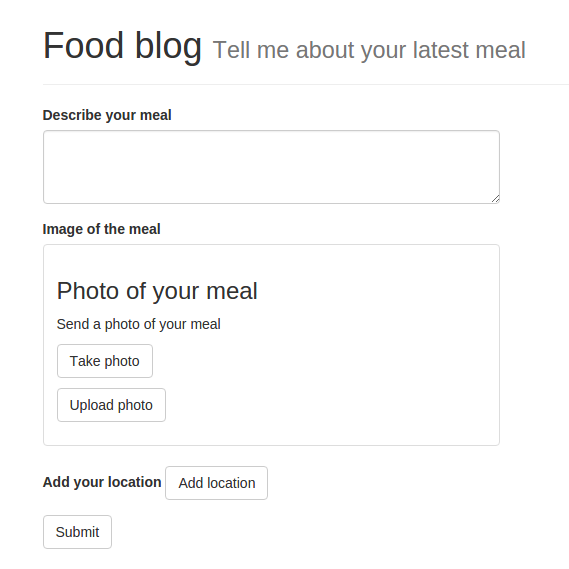
\includegraphics[width=120mm,natwidth=800,natheight=600]{./img/webAppFrontPage.png}
    \caption{The web app front page displayed in Google Chrome}
    \label{fig:webappfront}
\end{figure}

\subsection{The mobile application} \label{subsec:the-mobile-application}
The mobile application consists of two parts, the web application described above, and the mobile application encapsulating the web application. The mobile application must encapsulate the web application and display the web application the same way as it is displayed in a browser. The mobile application must use the mobile’s native functions to provide the web application with images and the mobiles location. The mobile application has no knowledge of the back-end of the web application, it merely communicates with the client-side of the web application (except for when requesting the front-end from the server).

The text field in the web application has no connection to the mobile application layer. 

For taking or uploading an image in the form, the mobile application must use an existing image from the image gallery or take a picture using the mobile camera. The photo must be passed back to the web application in Base64 format. 

The location must be obtained using the mobile’s GPS. 

When the user interacts with the mobile application, the interaction must be directly with the web application encapsulated within the mobile application. 

In the project the following equipment tools and programs were used for developing and testing:
\begin{itemize}
\item Version 21 of the Android SDK, when developing using the Android application framework
\item Apache Cordova CLI version 4.0, when developing using the PhoneGap framework
\item Android Studio, as the IDE when developing using the Android application framework
\item A regular text editor, for creating and editing JavaScript and HTML-files
\item A Nexus 5 mobile with the Android version 5.1.1, for testing the mobile applications
\item Google Chrome browser version 44.0.2403.157, for testing the web application
\end{itemize}

\section{Layer communication} \label{sec:layer-communication}
A prerequisite is that the communication between the mobile application and web application layer has a master and slave relationship. To evaluate this communication a flow diagram of the web layer sending a request for native data and the mobile application layer responding with data is constructed. The flow diagram acts as a suggestion in how developer friendly the communication is combined with our personal developing experiences.

\section{Measuring lines of code}\label{sec:measuring-lines-of-code}
The resulting mobile applications are measured using the software metric logical lines of code. To count logical lines of code Project Code Meter has been used which ignores the following lines of code~\cite{project-code-meter2015}

\begin{itemize}
\item Auto-generated code lines.
\item Header files.
\item Ineffective code statements.
\item Pragma compiler directives.
\item Labels.
\item Switch cases are not statements by themselves (so empty "case").
\item Several statements on the same physical line are counted as several LLOC.
\end{itemize}

The mobile application was written in two different programming languages, Java and JavaScript. To compare the measurement result of logical lines of code the conversion table described by Galorath and Evans~\cite[p.~163]{galorath2006} was used. JavaScript and Java are both third generation languages and therefore the conversion is roughly 1 to 1. 

The logical lines of code in the web application layer were also measured in both developing methods. The resulting lines in the mobile and web application layer were added together to give a total result. 